\section{Background and Related Work}
%\section{Preliminaries and Related Work}
\label{sec:bg}

\subsection{Emulating multi-port memories}
\label{sec:emulation}

Multi-port memory systems are essential for multi-core computation. Individual cores may request memory simulateously, and absent a multi-port memory system some cores will stall. Designing multi-port memory system has significant costs. Complex circuitry and large area requirements for multi-port bit-cells are significantly higher than those for single-port bit-cells~\cite{Suzuki,WLCH14}. This motivates the exploration of algorithmic and systematic designs that emulate multi-port memories using single-ported memory banks~\cite{ACP88, EMY91, RG91,Memoir_xor, Memoir_xor_virtual}. Attempts have been made to emulate multi-port memory using replication based designs \cite{CCES93}, however the resulting memory architectures are very large. \Ethan{Move some of this earlier?}

%\Ankit{This patent by  Chappell, Chappell, Ebcioglu and Schuster\cite{CCES93} arguing against both multi-port RAMs and their emulation using single-port RAMs. But the emulation is replication based so we can make a case here for coding based emulation.....}

\subsubsection{Read-only Support} 
\label{sec:read_only}
Replication-based designs are often proposed as a method for multi-port emulation. Suppose that a memory design is required to support only read requests, say $r$ read requests per memory clock cycle. A simple solution is storing $r$ copies of each data element on $r$ different single-port memory banks. In every memory clock cycle, the $r$ read requests can be served in a straightforward manner by mapping all read request to distinct memory banks (see Figure~\ref{fig:read_replication}). This way, the $r$-replication design completely avoids bank conflicts for up to $r$ read request in a memory clock cycle. 

\begin{remark}
\label{rem:read_only}
If we compare the memory design in Figure~\ref{fig:read_replication} with that of Figure~\ref{fig:example_xor}, we notice that both designs can simultaneously serve $2$ read requests without causing any bank conflicts. Note that the design in Figure~\ref{fig:example_xor} consumes smaller storage space as it needs only $3$ single-port memory banks while the design in  Figure~\ref{fig:read_replication} requires $4$ single-port memory banks. However, the access process for the design in Figure~\ref{fig:example_xor} involves some computation. {\color{red}This observation raises the notion that sophisticated coding schemes allow for storage efficient designs compared to replication based methods~\cite{MacSlo}. However, this comes at the expense of increased computation required for decoding.}
\end{remark}

%---------------------------
\begin{figure}[t!]
\centering
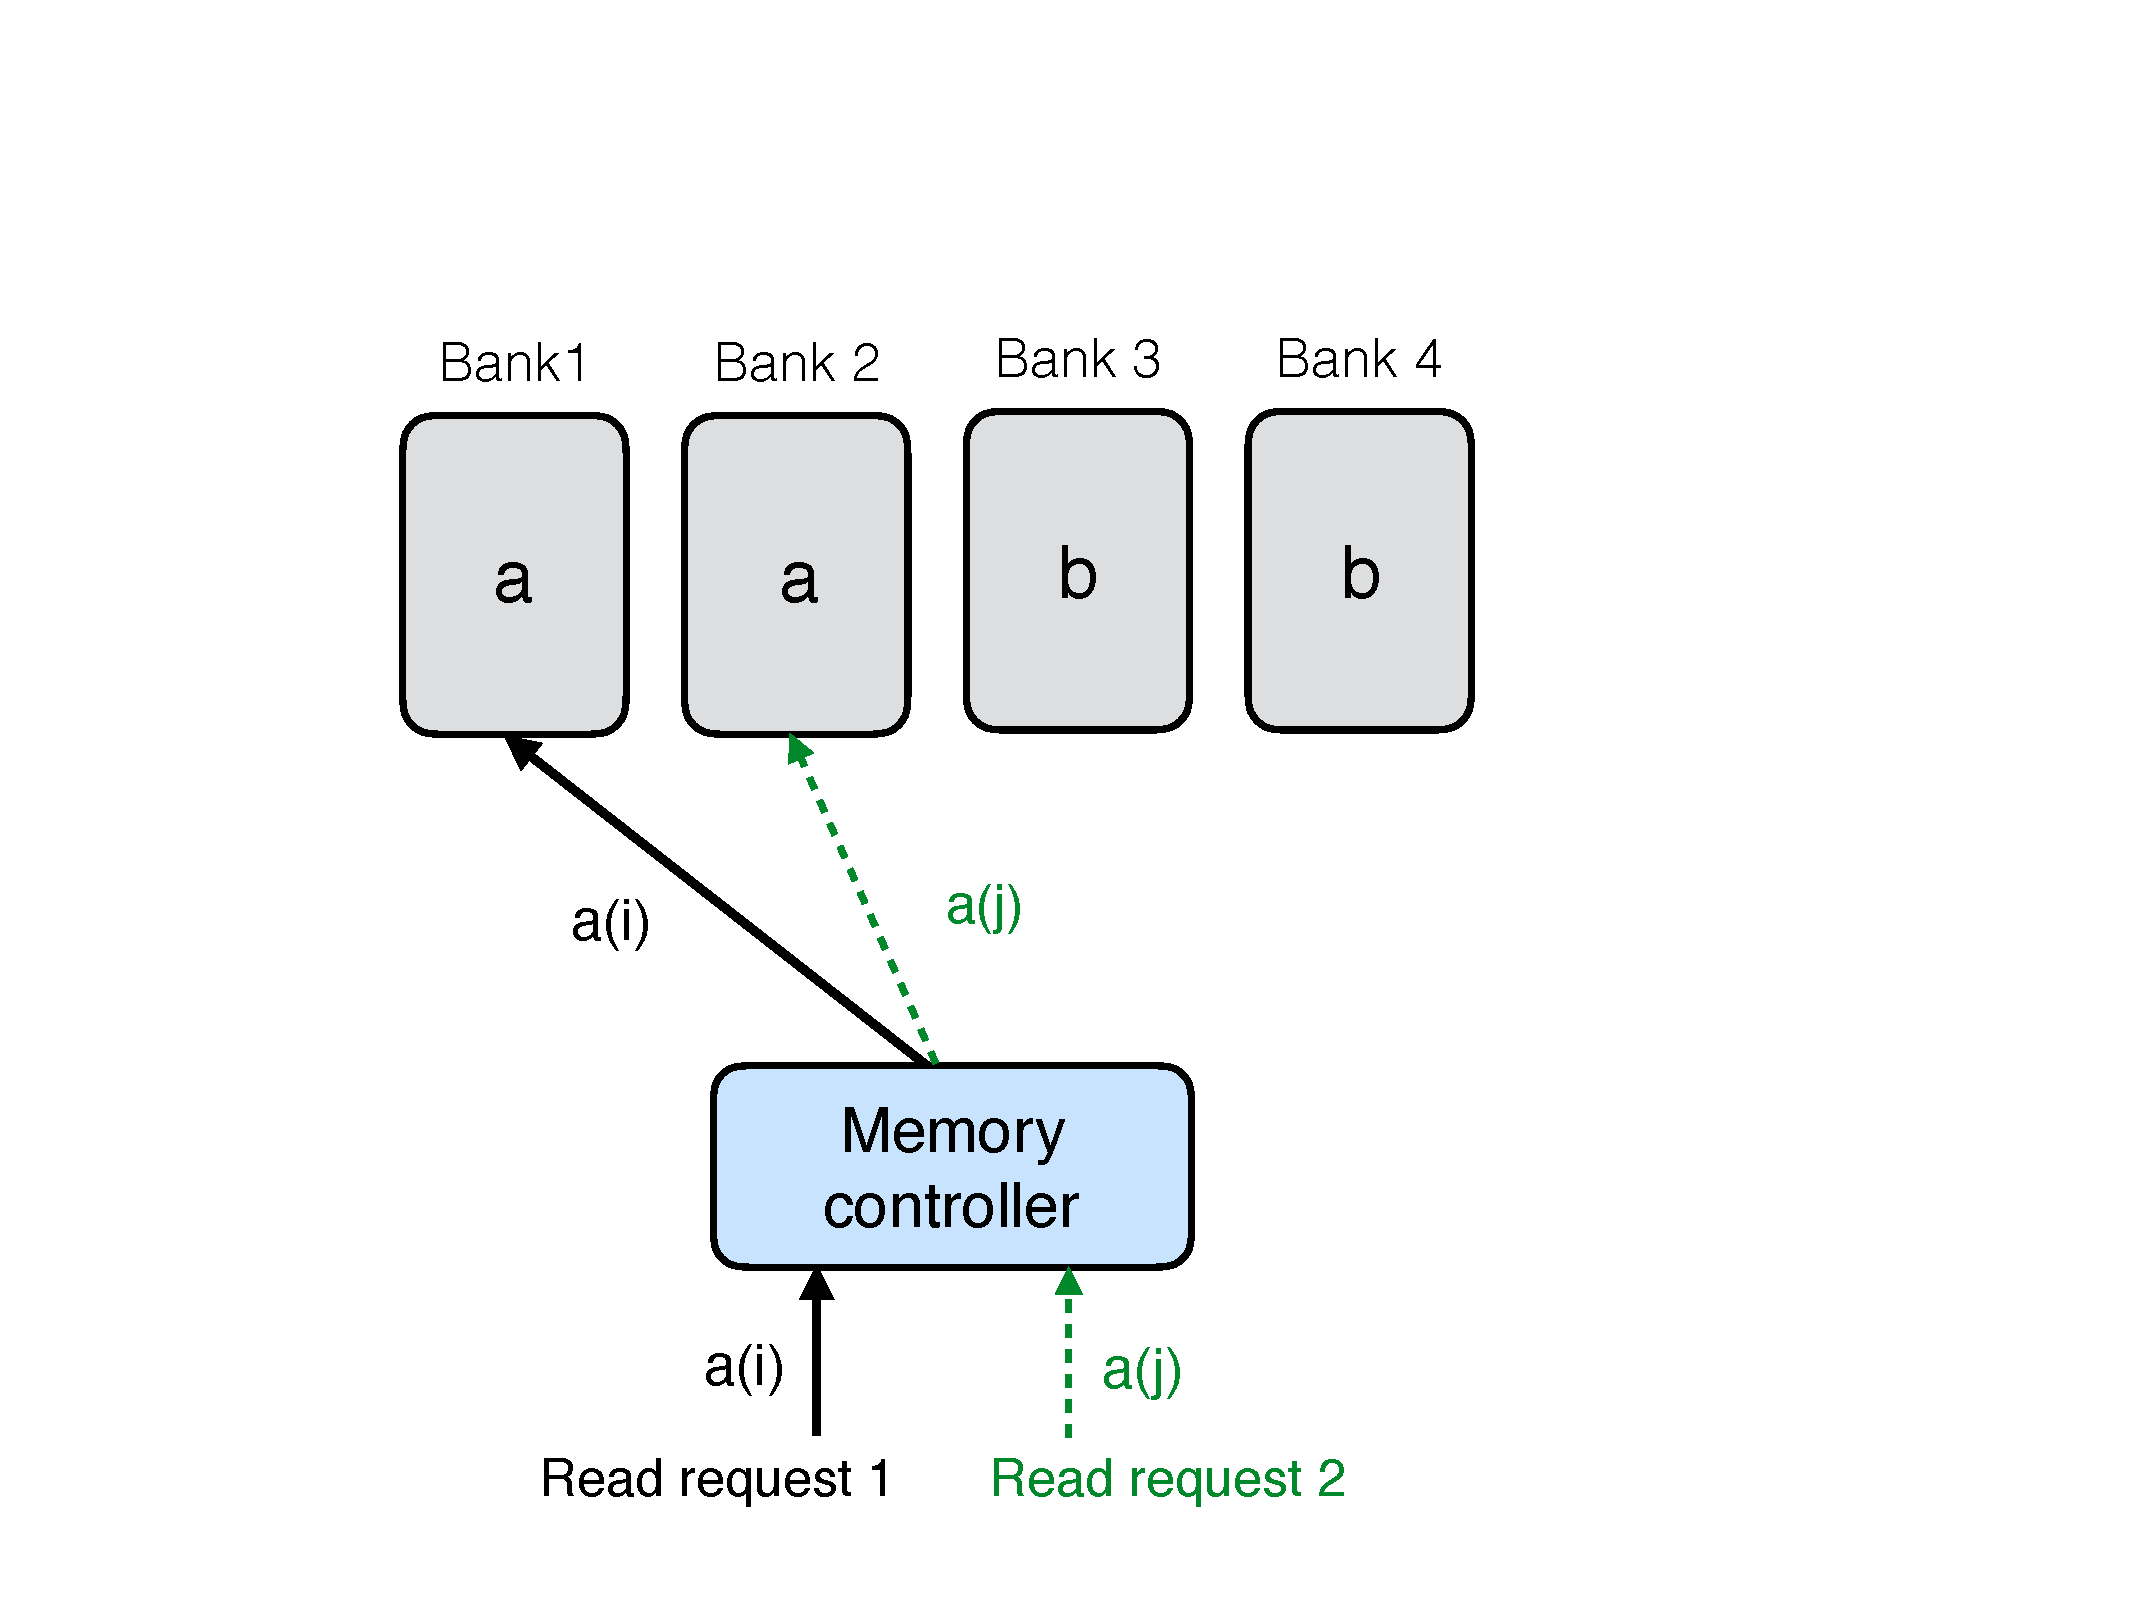
\includegraphics[width=0.425\linewidth]{fig/read-replication.pdf}
\caption{A $2$-replication design which supports $2$ read requests per bank. In this design, the data is partitioned between two banks $\mathbf{a} = [a(1),\ldots, a(L)]$ $\mathbf{b} = [b(1),\ldots, b(L)]$ and duplicated.}
\label{fig:read_replication}
\end{figure}
%---------------------------

%---------------------------
\begin{figure}[t!]
\centering
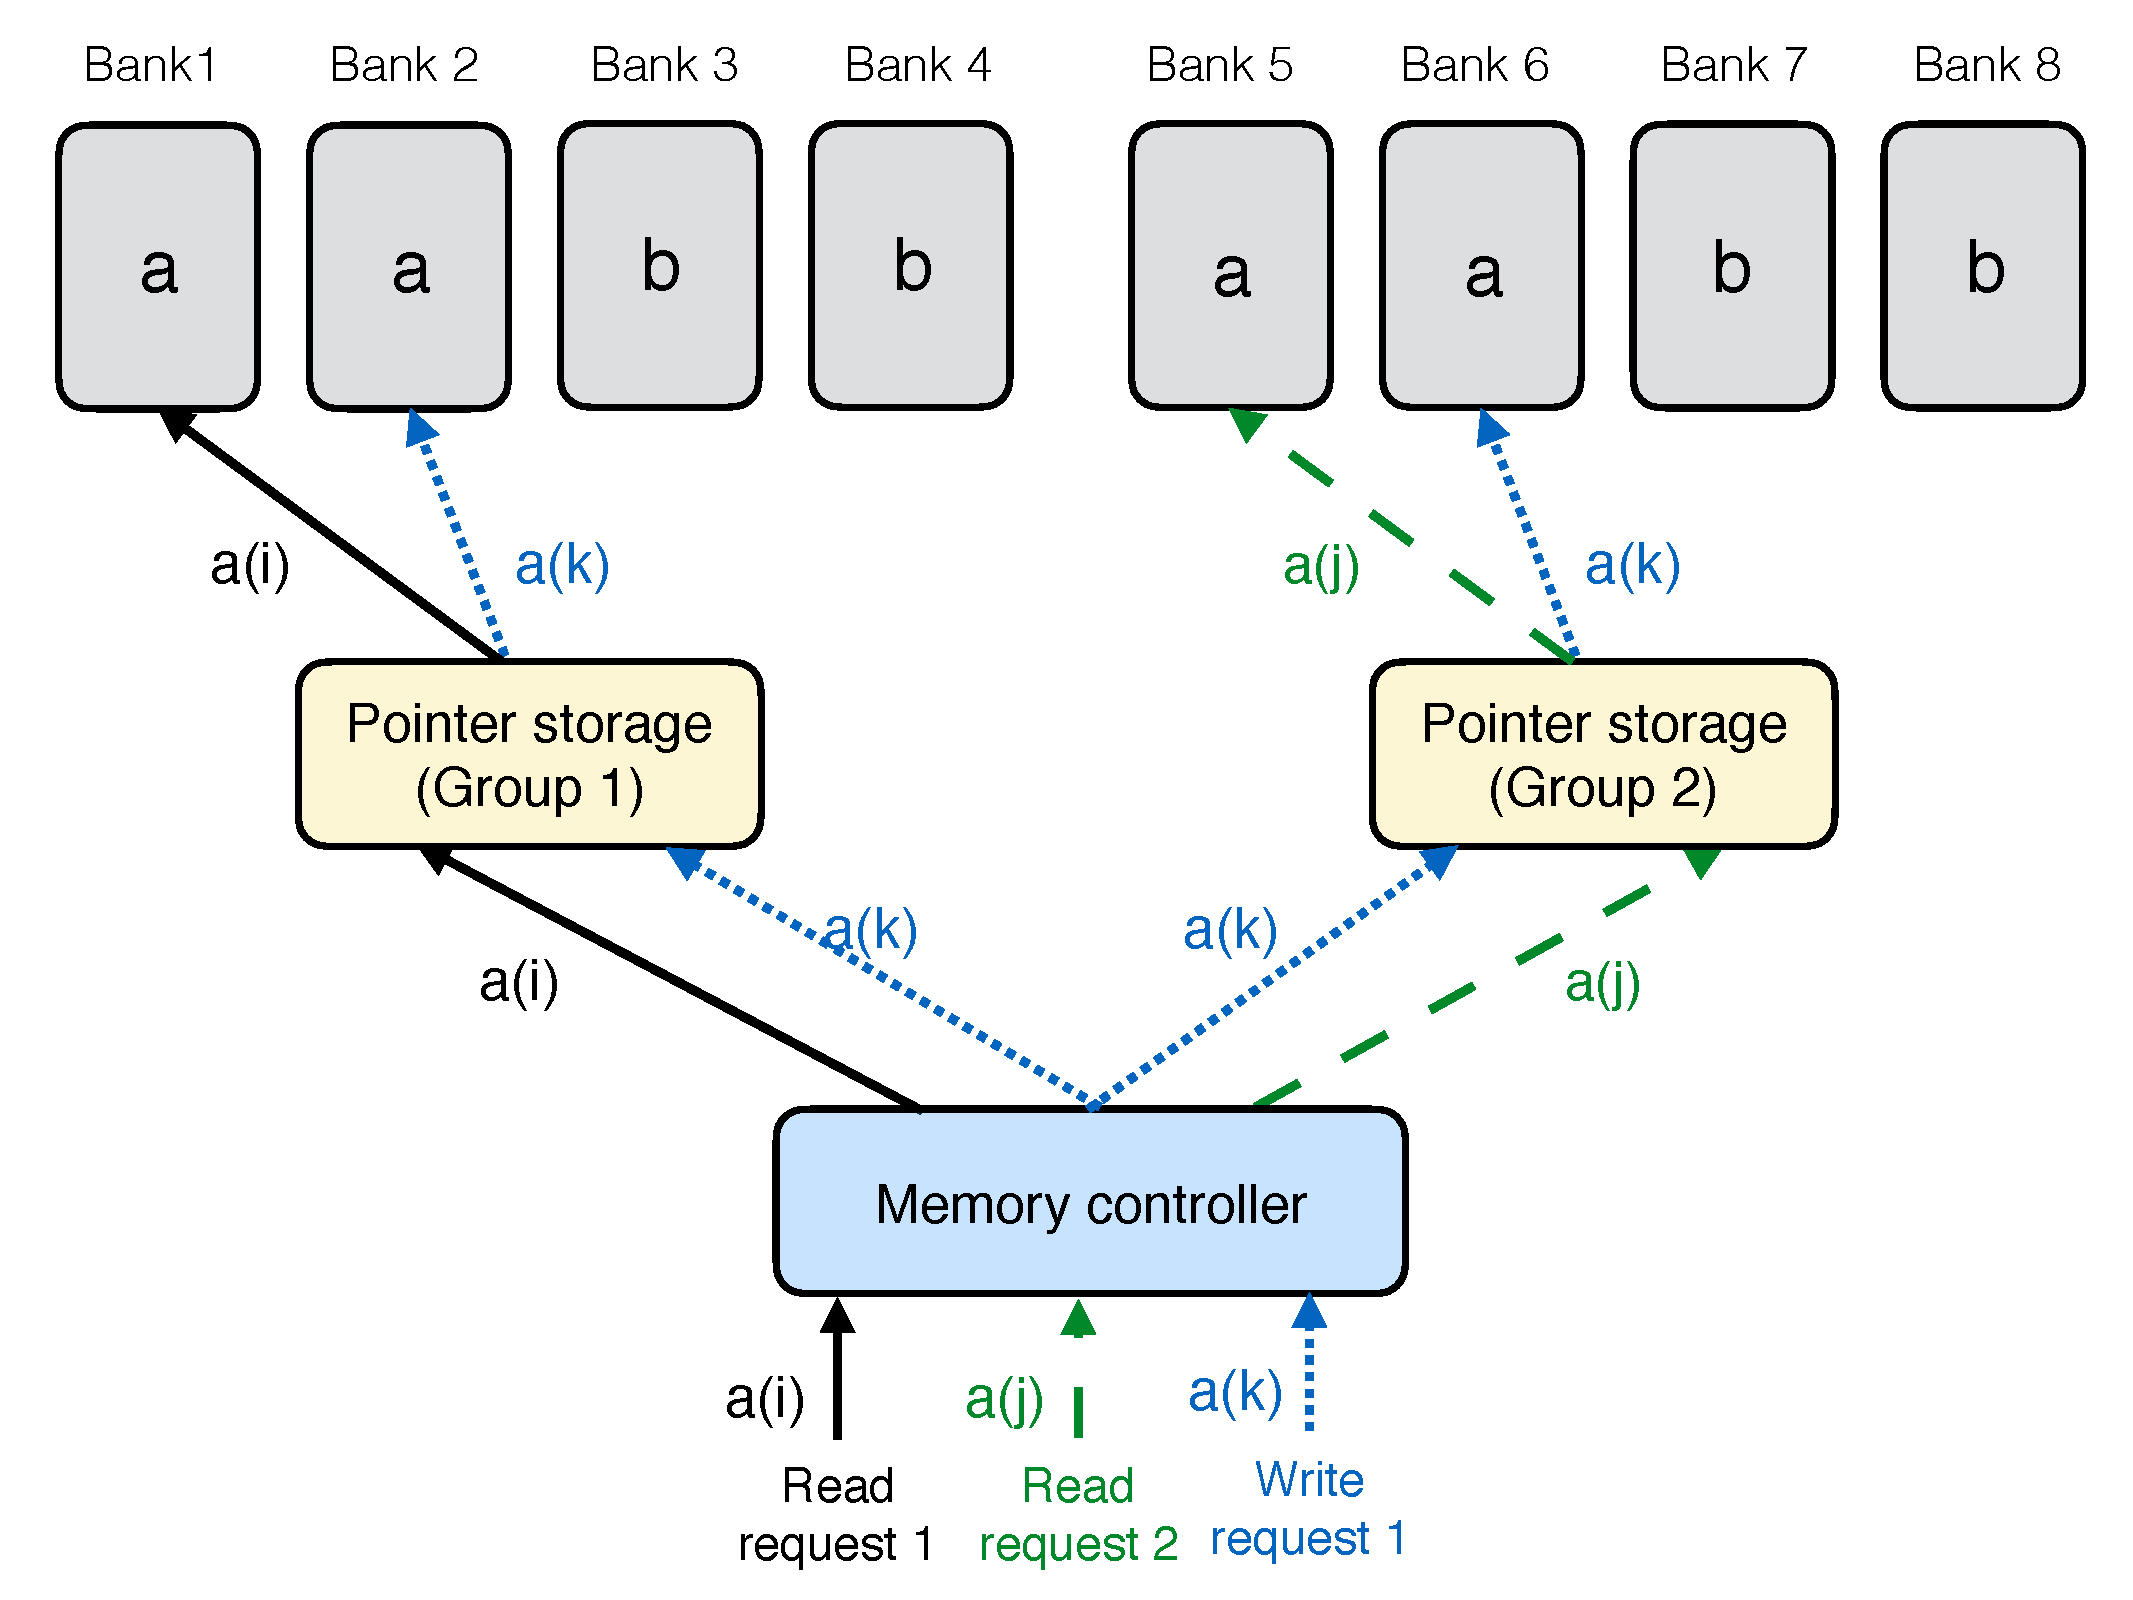
\includegraphics[width=0.86\linewidth]{fig/rw-replication.pdf}
\caption{A $4$-replication based design to support $r = 2$ read requests and $w = 1$ write requests. Both collections of information elements $\mathbf{a} = [a(1),\ldots, a(L)]$ and $\mathbf{b} = [b(1),\ldots, b(L)]$ are replicated to obtain $r\cdot (w + 1) = 4$ single-port memory banks. These banks are then partitioned into $r = 2$ disjoint groups, Banks $1$ -- $4$ and Banks $5$ -- $8$. 
Suppose that there are two read requests for $\{a(i), a(j)\}$ and a write request for $\{a(k)\}$. The memory architecture here enables the memory controller to schedule all three requests targeting bank $\mathbf{a}$ in the same memory cycle. The two read requests are served using one instance of bank $\mathbf{a}$ in each of the disjoint groups. The write request is served to one of the instances of $\mathbf{a}$ in each group. We serve the write requests to each disjoint group to ensure that each group contains up-to-date data. Each group must contain up-to-date data so that any arbitrary set of 2 read requests can be served by the two groups. As the write is served, the pointer storage is updated to keep track of the state of the data in the banks.}
\label{fig:rw_replication}
\end{figure}
%---------------------------
\subsubsection{Read and Write Support}
\label{sec:rw}
\Ankit{Mainly describing the results from the work of Auerbach, Chen, and  Paul\cite{ACP88}.} 
% It is evident from the discussion so far that we can indeed emulate the behavior of a multi-port memory on read requests by storing data on single-port memory banks in a redundant manner. 
A proper emulation of multi-port memory must be able to serve  write requests. A challenge that arises from this requirement is tracking the state of memory. In replication-based designs where original data banks are duplicated, the service of writes requests results in differences in state between the original and duplicate banks.

Replication-based solutions to the problems presented when supporting write requests involve creating yet more duplicate banks. A replication-based multi-port memory emulation that simultaneously supports $r$ read requests and $w$ write requests requires a $r\cdot(w + 1)$ replication scheme, where $r\cdot(w+1)$ copies of each data element are stored on $r\cdot(w + 1)$ different single-port memory banks. We illustrate this scheme for $r = 2$ and $w = 1$ in Figure~\ref{fig:rw_replication}. As in previous illustrations, we have two groups of symbols $\mathbf{a} = [a(1),\ldots, a(L)]$ and $\mathbf{b}  = [b(1),\ldots, b(L)]$. We store $4$ copies each of data elements $\mathbf{a}$ and $\mathbf{b}$ and partition the banks into $r = 2$ disjoint groups. Each group contains $(w + 1) = 2$ memory banks. An additional storage space, the pointer storage, is required keep track the state of the data in the banks.


%\subsection{Better emulation of multi-port memories}
\subsection{Storage-efficient emulation of multi-port memories}
\label{sec:efficient_emulation}

As described in Section~\ref{sec:emulation}, introducing redundancy to systems which use single-port memory banks allows such systems emulate the behavior of multi-port banks. In a setup where multi-port reads are supported (cf. Section~\ref{sec:read_only}) such emulation has little computational and storage cost. Emulating multi-port read and write systems is more costly (cf. Section~\ref{sec:rw}). A greater number of single-port memory banks are needed, and systems which redundantly store memory require tracking of the various versions of the data elements present in the memory banks. Furthermore, the presence of varying version of elements in the banks complicates the process of arbitration, as some memory banks may contain stale elements. Many programs in multi-core environments involve significant numbers of write requests, so any system which emulates multi-port memory using single-port memory must take these complications into account.

{\color{red}We believe that various tasks that arise in the presence of write requests and contribute to computational overhead of the memory design, including synchronization among memory banks and complicated arbitration, can be better managed at the algorithmic level.\Ethan{good point!} Note that these tasks are performed by the memory controller. It is possible to mitigate the effect of these tasks on the overall performance of memory system by relying on the increasing available computational resources while designing the memory controller. Additionally, we believe that large storage overhead is a more fundamental issue that needs to be addressed before the emulation of the multi-port memories is feasible. In particular, the large replication factor in a naive emulation create so large a storage overhead that the resulting area requirements of such designs are impractical.}

In order to reduce the storage overhead incurred by multi-port emulation, we avoid the native $r\cdot(w + 1)$-replication design. Another approach arises from the observation that some data banks are left unused during arbitration in individual memory cycles, while other data banks receive multiple requests. We encode the elements of the data banks using specific coding schemes to generate parity banks. Elements drawn from multiple data banks are encoded and stored in the parity banks. This approach allows us to utilize idle data banks to decode elements stored in the parity banks in service of multiple requests which target the same data bank. We recognize that this approach leads to increased complexity at the memory controller. {\color{red} {\em However, we show that the increase in complexity can be kept within an acceptable level while ensuring storage-efficient emulation of multi-port memories.}}

\subsection{Related work}

Coding theory is a well-studied field which aims to mitigate the challenges of underlying mediums in information processing systems ~\cite{MacSlo, Cover}. The field has enabled both reliable communication across noisy channel and reliability in fault-prone storage units. Recently, we have witnessed intensive efforts towards the application of coding theoretic ideas to design large scale distributed storage systems\cite{Azure, SAPDVCB13, Rashmi14}. In this domain of coding for distributed storage systems, the issue of access efficiency has also received attention, especially the ability to support multiple simultaneous read accesses with small storage overhead~\cite{batchcodes, RPDV16, RSDG16, Wang2017}. In this paper, we rely on such coding techniques to emulate multi-port memories using single-port memory banks. We note that the existing work on batch codes~\cite{batchcodes} focuses only on the read requests, but the emulation of multi-port memory must also handle write requests. 

Coding schemes with low update complexity that can be implemented at the speed memory systems require have also been studied ~\cite{ASV10, MCW14}). Our work is distinguished from the majority of the literature on coding for distributed storage, because we consider the interplay between read and write requests and how this interplay effects memory access latency.

In this paper, we also explore the idea of proactively prefetching the information from memory banks to improve the access efficiency of our memory design. The idea of prefetching in realizing fast data transfer between processors and memory has been previously explored in the literature (see \cite{Kim2016, Kadjo2014, Shevgoor2015, JL2013} and references therein). 
%However, our work addresses the issue of data prefetching in the context of coded memory system which is not addressed earlier in the literature. 
More recently, an LSTM-based recurrent neural network was used to predict future memory access requests on the SPEC 2006 benchmark dataset \cite{lstm2018}. This deep learning method may be used in addition to our proposed frequency-based approach.
Our combination of coded memory and prefetching also shares some similarity with the recent line of work on coded caching~\cite{MN16a} which aims to reduce the data downloaded from servers in a communication network by utilizing the cache available at the end users. Here, we would like to point out that there are many key differences in the our setup with coded memory banks with that considered in \cite{MN16a}. Our setup has data stored in an encoded form stored across memory banks and caching is enabled by the memory controller, which is a centralized unit. In contrast, the setup of coded caching has a centralized storage system (server) and cache units that store encoded information distributed across users.

{\color{red} {\bf The work which is closest to our solution for emulating a multi-port memory is by Iyer and Chuang~\cite{Memoir_xor, Memoir_xor_virtual}, where they also employ XORing based coding schemes to redundantly store information in an array of single-port memory banks. However, we note that our work significantly differers from \cite{Memoir_xor, Memoir_xor_virtual} as we specifically rely on different coding schemes arising under the framework of batch codes~\cite{batchcodes}. Additionally, due to the employment of distinct coding techniques, the design of memory controller in our work also differs from that in \cite{Memoir_xor, Memoir_xor_virtual}.}}

\Ankit{Also cite the work by Rivest et al.~\cite{RG91} and Endo, Matsumura and Yamada~\cite{EMY91}.}

%\section{Motivation}
%
%\subsection{Dual port RAM}
%
%\subsubsection{Replication}
%Because the size of the dual-ported SRAM bit-cell is almost double that of the single-ported SRAM bit-cell, a more versatile way (i.e., can do 2 reads in one cycle or one write) to implement dual-ported SRAM is by duplicating SRAM banks, as shown in Figure 3. In this way the bandwidth does not suffer from any loss for performing 2 simultaneous read operations, but only suffers 1 arbitration loss when performing simultaneous read and write operations (i.e., cannot perform 1 read and 1 write in the same cycle). The area is similar to that used in dual-ported circuit implementations. The advantage of this implementation is simplicity while the disadvantage is that if frequent write access is required the performance (bandwidth) is not as good as the true 1R1W SRAMs which can do a simultaneous read and write in one cycle.
%
%\subsubsection{Replication with pointer storage}
%
%Replication scheme $r + w$ replications...for $rRwW$ multipart memory.
%
%\subsubsection{Bank interleaving and arbitration}
%
%Another alternative is to use bank interleaving and arbitration circuits to allow for simultaneous access of different banks of memory. Occasional stalls are necessary in this approach if the arbitration circuit finds conflicting access to the same memory banks. Its operation is illustrated in Figure 4.
%
%Figure 4. Multiple accesses to SRAM by Bank interleaving with lower address bits. A large SRAM bank is sub-divided into n (n ? 2) smaller single-ported SRAM banks to support 2 or more simultaneous accesses. An arbitration unit is used in case conflicting addresses want to access the same bank, in which case one of the accesses is delayed.
%
%
%
%
%{\color{red}
%SRAMs can be categorized as single-ported or multi-ported. The single-ported SRAM is the most common type of SRAM with the best area efficiency and is used for most compiler memories due to its modular approach. Multi-ported memories are either not area efficient or with limited storage capability. Logical implementation of multi-ported memories with interleaved banks can be area efficient (because there is no memory duplication), but requires arbitration and flow-control circuits. Duplicating single-ported memory banks can support 2 reads and 1 write type of accesses with no additional delays and 1 read and 1 write type of access with 1.5 times the delay of read access;  Also its size is competitive relative to the true dual-ported memories. True multi-ported memories can be implemented with single-ported memories by replicating the memories multiple times. The area cost is r(w+1) times the number of bank replications.  Algorithmic approaches of multi-port memory design (such as Memoir) include caches and different ways of buffering of read and write data, with advantages being area efficiency and disadvantages including design complexity. Algorithmic memories can be statistical with lower areas or deterministic with higher areas, depending on the application.}

